\documentclass{article}
\usepackage{mathrsfs} % for scripts
\usepackage{standalone}
\usepackage{tikz}
\usetikzlibrary{arrows}
\usetikzlibrary{hobby}
\begin{document}
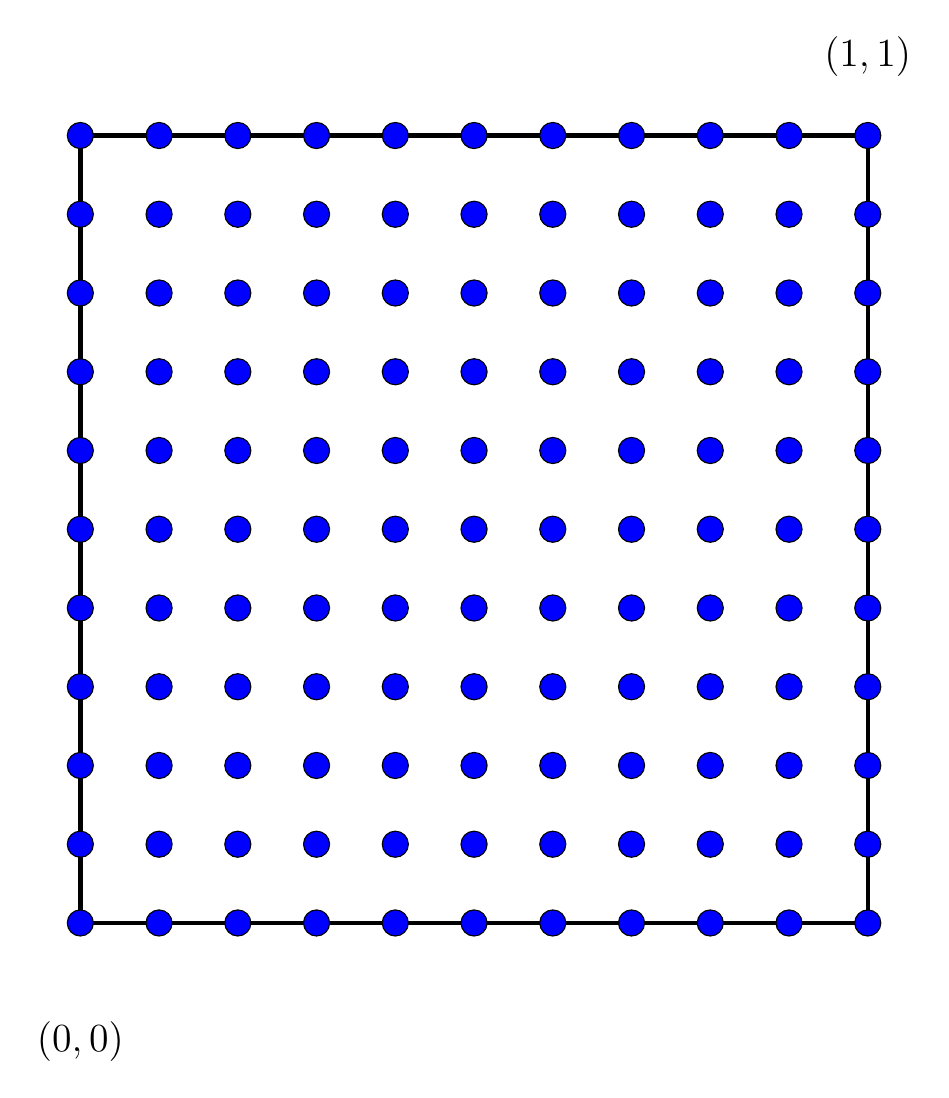
\begin{tikzpicture}[scale=10,darkstyle/.style={circle,draw,fill=gray!40,minimum size=01}]
    \begin{scope}
	\draw[{[-]}, ultra thick] (0,0) rectangle (1,1);
	\node at (0,-0.15) {\Large$(0,0)$};
	\node at (1,1.1) {\Large$(1,1)$};
	\foreach \x in {0,...,10}
	  \foreach \y in {0,...,10}
	    \node [circle,draw,fill=blue,minimum size=0.5]  (\x\y) at (0.1*\x,0.1*\y) {}; 
    \end{scope}
\end{tikzpicture}
\end{document}
